\documentclass[]{article}
\usepackage[portrait, margin=5mm]{geometry}
\usepackage{amsmath}
\usepackage{amssymb}
\usepackage{amsfonts}
\usepackage{listings}
\usepackage{graphicx}
\pagenumbering{gobble}

\renewcommand{\.}{\hskip .75pt}

\renewcommand{\arraystretch}{1.25}

\newcommand{\fin}[1]{[\.#1\.]}

\DeclareMathOperator{\aand}{\;\wedge\;}
\DeclareMathOperator{\st}{,\;}
\DeclareMathOperator{\ex}{\,\exists}

\let\r=\rightarrow
\let\*=\cdot

\begin{document}

\lstset{
	basicstyle=\ttfamily\small,
	literate=
	{→}{{$\rightarrow$}}1
	{∀}{{$\forall$}}1
	{∃}{{$\exists$}}1
	{×}{{$\times$}}1
	{σ}{{$\sigma$}}1
	{τ}{{$\tau$}}1
	{α}{{$\alpha$}}1
	{γ}{{$\gamma$}}1
	{≠}{{$\neq$}}1
	{≤}{{$\leq$}}1
	{≥}{{$\geq$}}1
	{↔}{{$\iff$}}1
	{¬}{{$\neg$}}1
	{∧}{{$\wedge$}}1
	{∨}{{$\vee$}}1
	{•}{$\bullet$}1
	{·}{$\cdot$}1
	{⬝}{$\cdot$}1
	{ℕ}{{$\mathbb{N}$}}1
	{ℤ}{{$\mathbb{Z}$}}1
	{ₗ}{{$_l$}}1
	{₀}{{$_0$}}1
	{∑}{{$\sum$}}1
	{ᵀ}{{$^\texttt{T}$}}1
	{ᵥ}{{$_v$}}1
	{ₘ}{{$_m$}}1
	{⁻¹}{{$^{-1}$}}1
	{∞}{{$\infty$}}1
	{⊤}{{$\top$}}1
	{⊥}{{$\bot$}}1
	{⟨}{{$\langle$}}1
	{⟩}{{$\rangle$}}1
	{∘}{{$\circ$}}1
}


\title{Duality theory in linear optimization and its extensions\:---\:formally verified}
\author{Martin Dvorak, Vladimir Kolmogorov}
\date{2024}
\maketitle


\noindent \textbf{Abstract:}\;
Farkas established that a system of linear inequalities has a solution if and only if we cannot obtain
a contradiction by taking a linear combination of the inequalities.
We state and formally prove several Farkas-like theorems in Lean 4.
Furthermore, we consider a linearly ordered field extended with two special elements denoted by $\bot$ and $\top$
where $\bot$ is below every element and $\top$ is above every element.
We define $\bot + a = \bot = a + \bot$ for all $a$ and we define $\top + b = \top = b + \top$ for all $b \neq \bot$.
Instead of multiplication, we define scalar action $c \bullet \bot = \bot$ for every $c \ge 0$ but we define
$d \bullet \top = \top$ only for $d > 0$ because $0 \bullet \top = 0$.
We extend certain Farkas-like theorems to a setting where coefficients are from an extended linearly ordered field.


\section{Introduction}

We do not use set theory.
We write everything in type theory.
Juxtaposition never denotes multiplication.
Juxtaposition is always function application.
We often talk about linearly ordered fields.
The two main examples are rationals and reals.
The paper starts with famous corollaries and
then proceeds to state more general theorems.
Proofs are postponed to respective sections.
Theorems come with names instead of numbers.

There are two famous theorems characterizing that a system of linear inequalities
has a solution if and only if we cannot obtain a contradiction
by taking a linear combination of the inequalities.
TODO cite Farkas.

\medskip \noindent
\textbf{Theorem (equalityFarkas):}
Let $I$ and $J$ be finite types.
Let $F$ be a linearly ordered field.
Let $A$ be a matrix of type $(I \times J) \r F$.
Let $b$ be a vector of type $I \r F$.
Exactly one of the following exists:
\begin{itemize}
\item nonnegative vector $x : J \r F$ such that $A \* x = b$
\item vector $y : I \r F$ such that $A^T\! \* y \ge 0$ and $b \* y < 0$
\end{itemize}
TODO cite Minkowski?

\medskip \noindent
\textbf{Theorem (inequalityFarkas):}
Let $I$ and $J$ be finite types.
Let $F$ be a linearly ordered field.
Let $A$ be a matrix of type $(I \times J) \r F$.
Let $b$ be a vector of type $I \r F$.
Exactly one of the following exists:
\begin{itemize}
\item nonnegative vector $x : J \r F$ such that $A \* x \le b$
\item nonnegative vector $y : I \r F$ such that $A^T\! \* y \ge 0$ and $b \* y < 0$
\end{itemize}
TODO cite John von Neumann?
(any maybe Oskar Morgenstern and maybe George Dantzig and maybe Albert W. Tucker?)

\medskip \noindent
\textbf{Theorem (StandardLP.strongDuality):}
Let $I$ and $J$ be finite types.
Let $F$ be a linearly ordered field.
Let $A$ be a matrix of type $(I \times J) \r F$.
Let $b$ be a vector of type $I \r F$.
Let $c$ be a vector of type $J \r F$.
Then
$$ \min \,\{\, c \* x ~|~ x \ge 0 \aand A \* x \le b \,\}
=- \min \,\{\, b \* y ~|~ y \ge 0 \aand A^T\! \* y \le c \,\}
$$
holds if at least one of the systems has a solution
(very roughly paraphrased\:---\:this is not how our theorem is stated).


\subsection{Structure of this paper}

In Section 1.1, we generalize equalityFarkas to a broader
linear-algebraic setting.
In Section 1.2, we generalize inequalityFarkas and
StandardLP.strongDuality to structures that allow
infinite values in certain places.
In Section 2, we comment on the formalization process.
In Section 3, we prove the theorem from Section 1.1,
from which be obtain equalityFarkas as a corollary.
In Section 4, we prove the extension of inequalityFarkas.
In Section 5, we prove the strong duality theorem from
Section 1.2, from which we obtain
StandardLP.strongDuality as a corollary.

Repository \texttt{https://github.com/madvorak/duality}
contains full version of all definitions, statements,
and proofs. They are written in a formal language called
Lean 4, which provides a guarantee that every step of
every proof follows from valid logical axioms.\footnote{
The only axioms used in our proofs are
propext, Classical.choice, and Quot.sound, which you can
check by the \texttt{\#print axioms} command.}
This paper attempts to be an accurate description of
the \texttt{duality} project.
However, in case of any discrepancy, the code shall prevail.


\subsection{Generalizations}

The next theorem generalizes equalityFarkas to structures where
multiplication does not have to be commutative.
Furthermore, it supports infinitely many equations.
\pagebreak[2]

\medskip \noindent
\textbf{Theorem (coordinateFarkas):}
Let $I$ be any type.
Let $J$ be a finite type.
Let $R$ be a linearly ordered division ring.
Let $A$ be an $R$-linear map from from $(I \r R)$ to $(J \r R)$.
Let $b$ be an $R$-linear map from from $(I \r R)$ to $R$.
Exactly one of the following exists:
\begin{itemize}
\item nonnegative vector $x : J \r R$ such that, for all $w : I \r R$, we have
$ \sum_{j : J}\; (A~w)_j \bullet x_j = b~w $
\item vector $y : I \r R$ such that $A~y \ge 0$ and $b~y < 0$
\end{itemize}
In the next generalization, we replace the partially ordered module $I \r R$ by
a general $R$-module $W$.

\medskip \noindent
\textbf{Theorem (scalarFarkas):}
Let $J$ be a finite type.
Let $R$ be a linearly ordered division ring.
Let $W$ be an $R$-module.
Let $A$ be an $R$-linear map from from $W$ to $(J \r R)$.
Let $b$ be an $R$-linear map from from $W$ to $R$.
Exactly one of the following exists:
\begin{itemize}
\item nonnegative vector $x : J \r R$ such that, for all $w : W$, we have
$ \sum_{j : J}\; (A~w)_j \bullet x_j = b~w $
\item vector $y : W$ such that $A~y \ge 0$ and $b~y < 0$
\end{itemize}
In the most general theorem, stated below, we replace certain occurrences of $R$ by
a linearly ordered $R$-module $V$ whose order respects order on $R$.
This result origins from TODO cite Bartl.

\medskip \noindent
\textbf{Theorem (fintypeFarkasBartl):}
Let $J$ be a finite type.
Let $R$ be a linearly ordered division ring.
Let $W$ be an $R$-module.
Let $V$ be a linearly ordered $R$-module.
Let $A$ be an $R$-linear map from $W$ to $(J \r R)$.
Let $b$ be an $R$-linear map from $W$ to $V$.
Exactly one of the following exists:
\begin{itemize}
\item nonnegative vector family $x : J \r V$ such that, for all $w : W$, we have
$ \sum_{j : J}\; (A~w)_j \bullet x_j = b~w $
\item vector $y : W$ such that $A~y \ge 0$ and $b~y < 0$
\end{itemize}
In the last branch, $A~y \ge 0$ uses the partial order on $(J \r R)$ whereäs
$b~y < 0$ uses the linear order on $V$.
Note that fintypeFarkasBartl subsumes scalarFarkas (as well as the other versions based on equality),
since $R$ can be viewed as a linearly ordered module over itself.
We prove fintypeFarkasBartl in Section 3, which is where the heavy lifting comes.


\subsection{Extensions}

Until now, we have talked about known results.
What follows is a new extension of the theory.

\medskip \noindent
\textbf{Definition:}
Let $F$ be a linearly ordered field.
We define an \textbf{extended} linearly ordered field $F_\infty$ as
$F \cup \{ \bot, \top \}$ with the following properties.
Let $p$ and $q$ be numbers from $F$.
We have $\bot < p < \top$.
We define addition, scalar action, and negation on $F_\infty$ as follows:
\begin{center}
	\begin{tabular}{ c || c | c | c | }
		+ & $\bot$ & $q$ & $\top$  \\
		\hline\hline
		$\bot$ & $\bot$ & $\bot$ & $\bot$  \\ 
		\hline
		$p$ & $\bot$ & $p\!+\!q$ & $\top$  \\ 
		\hline
		$\top$ & $\bot$ & $\top$ & $\top$ \\ 
		\hline
	\end{tabular}
	\qquad\qquad\qquad
	\begin{tabular}{ c || c | c | c | }
		$\bullet$ & $\bot$ & $q$ & $\top$  \\
		\hline\hline
		$0$ & $\bot$ & $0$ & $0$  \\ 
		\hline
		$p>0$ & $\bot$ & $p \cdot q$ & $\top$  \\ 
		\hline
	\end{tabular}
	\qquad\qquad\qquad
	\begin{tabular}{ c || c | c | c }
	$-$ & $\bot$ & $q$ & $\top$  \\
	\hline\hline
	& $\top$ & $-q$ & $\bot$  
	\end{tabular}
\end{center}
When we talk about elements of $F_\infty$,
we say that values from $F$ are \textbf{finite}.

Informally speaking, $\top$ represents the positive infinity,
$\bot$ represents the negative infinity, and we say that
$\bot$ is ``stronger'' than $\top$ in~all arithmetic operations.
The surprising parts are $\bot + \top = \bot$ and $0 \.\bullet \bot = \bot$.
Because of them, $F_\infty$ is not a field.
In fact, $F_\infty$ is not even a group. 
However, $F_\infty$ is still a densely linearly ordered abelian monoid
with characteristic zero.

\medskip \noindent
\textbf{Theorem (extendedFarkas):}
Let $I$ and $J$ be finite types.
Let $F$ be a linearly ordered field.
Let $A$ be a matrix of type $(I \times J) \r F_\infty$.
Let $b$ be a vector of type $I \r F_\infty$.
Assume that $A$ does not have $\bot$ and $\top$ in the same row.
Assume that $A$ does not have $\bot$ and $\top$ in the same column.
Assume that $A$ does not have $\top$ in any row where $b$ has $\top$.
Assume that $A$ does not have $\bot$ in any row where $b$ has~$\bot$.
Exactly one of the following exists:
\begin{itemize}
\item nonnegative vector $x : J \r F$ such that $A \* x \le b$
\item nonnegative vector $y : I \r F$ such that $(-A^T) \* y \le 0$ and $b \* y < 0$
\end{itemize}
Note that extendedFarkas looks pretty much like equalityFarkas\_neg and,
in certain sense, generalizes it. Indeed, in Section 4, we prove
extendedFarkas using equalityFarkas\_neg and some additional machinery.
TODO rephrase without mentioning equalityFarkas\_neg.

Next we define an extended notion of linear program, i.e.,
linear programming over extended linearly ordered fields.
The implicit intention is that the linear program is to be minimized.

\medskip \noindent
\textbf{Definition:}
Let $I$ and $J$ be finite types.
Let $F$ be a linearly ordered field.
Let $A$ be a matrix of type $(I \times J) \r F_\infty$,
let $b$ be a vector of type $I \r F_\infty$,
and $c$ be a vector of type $J \r F_\infty$
such that the following six conditions hold:
\begin{itemize}
\item $A$ does not have $\bot$ and $\top$ in the same row
\item $A$ does not have $\bot$ and $\top$ in the same column
\item $b$ does not contain $\bot$
\item $c$ does not contain $\bot$
\item $A$ does not have $\top$ in any row where $b$ has $\top$
\item $A$ does not have $\bot$ in any column where $c$ has $\top$
\end{itemize}
We say that $P = (A, b, c)$ is a \textbf{linear program} over $F_\infty$
whose constraints are indexed by $I$ and variables are indexed by $J$.
We say that a nonnegative vector $x : J \r R$ is
a \textbf{solution} to $P$ if and only if $A \* x \le b$.
We say that $P$ \textbf{reaches} an objective value $r$
if and only if there exists $x$ such that $x$ is a solution to $P$
and $c \* x = r$.
We say that $P$ is \textbf{feasible} if and only if $P$ reaches a finite\footnote{
It would be perhaps more natural to say that $P$ reaches a value different
from $\top$. However, since $\bot$ cannot be reached because of the way
linear programming is defined, it is equivalent to our definition by
reaching a finite value.} value.
We say that $P$ is \textbf{bounded by} a finite value $r$ if and only if,
for every value $p$ reached by $P$, we have $r \le p$.
We say that $P$ is \textbf{unbounded} if and only if there is no finite value $r$
such that $P$ is bounded by $r$.
We say that the linear program $(-A^T, c, b)$ is the \textbf{dual} of $P$.

\medskip \noindent
\textbf{Theorem (ExtendedLP.weakDuality):}
Let $F$ be a linearly ordered field.
Let $P$ be a linear program over $F_\infty$.
If $P$ reaches $p$ and the dual of $P$ reaches $q$,
then $p + q \ge 0$.

\medskip \noindent
\textbf{Definition:}
Let $F$ be a linearly ordered field.
Let $P$ be a linear program over $F_\infty$.
We define the \textbf{optimum} of $P$ as follows.
If $P$ is feasible and unbounded, its optimum is $\bot$.
If $P$ is not feasible, its optimum is $\top$.
In all other cases, we ask whether $P$ reaches a finite value $r$ such that
$P$ is bounded by $r$. If so, its optimum is $r$.
Otherwise, $P$ does not have optimum.\footnote{By the end of the paper, we will
have proved that optimum always exists, i.e., it cannot happen that the set of
objective values reached by $P$ has a finite infimum that is not attained.
However, because we do not have the theorem now, the optimum is defined as a partial function
from linear programs to $F_\infty$.}

\medskip \noindent
\textbf{Theorem (ExtendedLP.strongDuality):}\footnote{For simplicity,
we rephrased the theorem without mentioning partial functions.
Also note that it would be incorrect to say the following:
$P$ has optimum~$p$, the dual of $P$ has optimum $q$, and $p + q = 0$.
It would fail for unbounded linear programs because the arithmetics
of $F_\infty$ defines $\top + \bot = \bot$.}
Let $F$ be a linearly ordered field.
Let $P$ be a linear program over $F_\infty$.
If $P$ or its dual is feasible (at least one of them),
then there exists $p$ in $F_\infty$ such that
$P$ has optimum $p$ and the dual of $P$ has optimum $-p$.

\section{Formalization}

\subsection{We start with a review of algebraic typeclasses that our project depends on}

Additive semigroup is a structure on any type with addition where the addition is associative:
\begin{lstlisting}
class AddSemigroup (G : Type u) extends Add G where
  add_assoc : ∀ a b c : G, (a + b) + c = a + (b + c)
\end{lstlisting}
Additive monoid is an additive semigroup with the zero element, thanks to which we can
define a scalar multiplication by the natural numbers (TODO AddZeroClass):
\begin{lstlisting}
class AddMonoid (M : Type u) extends AddSemigroup M, AddZeroClass M where
  nsmul : ℕ → M → M
  nsmul_zero : ∀ x : M, nsmul 0 x = 0 
  nsmul_succ : ∀ (n : ℕ) (x : M), nsmul (n + 1) x = nsmul n x + x 
\end{lstlisting}
Subtractive monoid is an additive monoid that adds two more operations (unary and binary minus)
that satisfy some basic properties:
\begin{lstlisting}
class SubNegMonoid (G : Type u) extends AddMonoid G, Neg G, Sub G where
  sub := SubNegMonoid.sub'
  sub_eq_add_neg : ∀ a b : G, a - b = a + -b 
  zsmul : ℤ → G → G
  zsmul_zero' : ∀ a : G, zsmul 0 a = 0 
  zsmul_succ' (n : ℕ) (a : G) : zsmul (Int.ofNat n.succ) a = zsmul (Int.ofNat n) a + a
  zsmul_neg' (n : ℕ) (a : G) : zsmul (Int.negSucc n) a = -(zsmul n.succ a)
\end{lstlisting}
Additive group is a subtractive monoid in which the unary minus acts as an inverse with respect to addition:
\begin{lstlisting}
class AddGroup (A : Type u) extends SubNegMonoid A where
  add_left_neg : ∀ a : A, -a + a = 0
\end{lstlisting}
Abelian group is defined as an additive group that is a commutative additive monoid at the same time (TODO AddCommMonoid):
\begin{lstlisting}
class AddCommGroup (G : Type u) extends AddGroup G, AddCommMonoid G
\end{lstlisting}
Ring is defined as a semiring that is an abelian group at the same time and has 1 that behaves well (TODO Semiring):
\begin{lstlisting}
class Ring (R : Type u) extends Semiring R, AddCommGroup R, AddGroupWithOne R
\end{lstlisting}
Division ring is a ring with a lot of extra requirements (TODOs DivInvMonoid, Nontrivial, NNRatCast, RatCast):
\begin{lstlisting}
class DivisionRing (α : Type*) extends Ring α, DivInvMonoid α, Nontrivial α, NNRatCast α, RatCast α where
  mul_inv_cancel : ∀ (a : α), a ≠ 0 → a * a⁻¹ = 1
  inv_zero : (0 : α)⁻¹ = 0
  nnratCast := NNRat.castRec
\end{lstlisting}
We define a linearly ordered division ring as a division ring that is a linearly ordered ring at the same time (TODO all about order):
\begin{lstlisting}
class LinearOrderedDivisionRing (R : Type*) extends LinearOrderedRing R, DivisionRing R
\end{lstlisting}
Linearly ordered field is defined as a linearly ordered commutative ring that is a field at the same time (TODO Field):
\begin{lstlisting}
class LinearOrderedField (α : Type*) extends LinearOrderedCommRing α, Field α
\end{lstlisting}
Note that LinearOrderedDivisionRing is not a part of the algebraic hierarchy provided by Mathlib,
hence LinearOrderedField does not inherit LinearOrderedDivisionRing, thus we provide a custom
instance that converts LinearOrderedField to LinearOrderedDivisionRing:
\begin{lstlisting}
instance LinearOrderedField.toLinearOrderedDivisionRing {F : Type*} [instF : LinearOrderedField F] :
  LinearOrderedDivisionRing F := { instF with }
\end{lstlisting}
This instance is needed for the step from coordinateFarkas to equalityFarkas.

\subsection{Extended linearly ordered fields}

Given any type $F$, we construct $F \cup \{ \bot, \top \}$ as follows:
\begin{lstlisting}
def Extend (F : Type*) := WithBot (WithTop F)
\end{lstlisting}
From now on we assume that $F$ is a linearly ordered field:
\begin{lstlisting}
variable {F : Type*} [LinearOrderedField F]
\end{lstlisting}
The following instance defines how addition and comparison
behaves on $F_\infty$ and automatically generates a proof
that $F_\infty$ forms a linearly ordered abelian monoid:
\begin{lstlisting}
instance : LinearOrderedAddCommMonoid (Extend F) :=
  inferInstanceAs (LinearOrderedAddCommMonoid (WithBot (WithTop F)))
\end{lstlisting}
The following definition embeds $F$ in $F_\infty$ and registers
this canonical embedding as a type coercion:
\begin{lstlisting}
@[coe] def toE : F → (Extend F) := some ∘ some
instance : Coe F (Extend F) := ⟨toE⟩
\end{lstlisting}
Unary minus on $F_\infty$ is defined as follows:
\begin{lstlisting}
def neg : Extend F → Extend F
| ⊥ => ⊤
| ⊤ => ⊥
| (x : F) => toE (-x)
instance : Neg (Extend F) := ⟨EF.neg⟩
\end{lstlisting}
In the file \texttt{FarkasSpecial.lean} and everything downstream,
we have the notation
\begin{lstlisting}
F∞
\end{lstlisting}
for $F_\infty$ and also the notation
\begin{lstlisting}
F≥0
\end{lstlisting}
for all nonnegative elements of $F$.
TODO define scalar action and explain SMulZeroClass.

\subsection{Vectors and matrices}

We distinguish two types of vectors; implicit vectors and explicit vectors.
Implicit vectors are members of a vector space; they don't have any internal structure.
Explicit vectors are functions from coordinates to values.
The set of coordinates needn't be ordered.
Matrices live next to explicit vectors. They are also functions; they take a row index
and a column index and they output a value at the given spot.
Neither the row indices nor the column vertices are required to form an ordered set.
That's why multiplication between matrices and vectors is defined only in structures
where addition forms a commutative semigroup. Consider the following example:
$$
\begin{pmatrix}
	1 & 2 & 3 \\
	4 & 5 & 6 \\
\end{pmatrix}
\*
\begin{pmatrix}
	7 \\ 8 \\ 9
\end{pmatrix}
=
\begin{pmatrix}
	? \\ \_
\end{pmatrix}
$$
We don't know whether the value at the question mark is equal to
$ (1 \* 7 + 2 \* 8) + 3 \* 9 $ or to
$ (2 \* 8 + 1 \* 7) + 3 \* 9 $ or to
any other ordering of summands.
This is why commutativity of addition is necessary for the definition to be valid.
On the other hand, we don't assume any property of multiplication in the
definition of multiplication between matrices and vectors; they don't even
have to be of the same type; we only require the elements of the vector
to have an action on the elements of the matrix (this is not a typo\:---\:normally,
we would want matrices to have an action on vectors\:---\:not in our work).

\subsubsection{Mathlib definitions versus our definitions}

Mathlib defines dot product (i.e., a product of an explicit vector with an explicit vector) as follows:
\begin{lstlisting}
def Matrix.dotProduct [Fintype m] [Mul α] [AddCommMonoid α] (v w : m → α) : α :=
  ∑ i, v i * w i
\end{lstlisting}
Mathlib defines a product of a matrix with an explicit vector as follows:
\begin{lstlisting}
def Matrix.mulVec [Fintype n] [NonUnitalNonAssocSemiring α] (M : Matrix m n α) (v : n → α) : m → α
  | i => (fun j => M i j) ⬝ᵥ v
\end{lstlisting}
Mildly confusingly, \texttt{m} and \texttt{n} are type variables here, not natural numbers.
Note that, when multiplying two vectors,
the left vector is not transposed\:---\:a vector is not
defined as a special case of matrix, and transposition is not
defined as an operation on explicit vectors, only on matrices.

Infix notation for these two operations is defined as follows
(the keyword \texttt{infixl} when defining an operator $\circ$ means that
\hbox{\texttt{x $\circ$ y $\circ$ z}} gets parsed as \texttt{(x $\circ$ y) $\circ$ z}
whether or not it makes sense, whereäs the keyword \texttt{infixr} when defining an operator $\circ$ means that %lb
\hbox{\texttt{A $\circ$ B $\circ$ v}} gets parsed as \texttt{A $\circ$ (B $\circ$ v)}
whether or not it makes sense):
\begin{lstlisting}
scoped infixl:72 " ⬝ᵥ " => Matrix.dotProduct
scoped infixr:73 " *ᵥ " => Matrix.mulVec
\end{lstlisting}
These definitions are sufficient for stating results based on linearly ordered fields.
However, our results from Section 1.3 require a more general notion of multiplication
between matrices and vectors.
They are defined in the section hetero\_matrix\_products\_defs as follows:
\begin{lstlisting}
variable {α γ : Type*} [AddCommMonoid α] [SMul γ α]

def Matrix.dotProd (v : I → α) (w : I → γ) : α :=
  ∑ i : I, w i • v i
infixl:72 " ᵥ⬝ " => Matrix.dotProd

def Matrix.mulWeig (M : Matrix I J α) (w : J → γ) (i : I) : α :=
  M i ᵥ⬝ w
infixr:73 " ₘ* " => Matrix.mulWeig
\end{lstlisting}
We start by declaring that $\alpha$ and $\gamma$ are types from
any universe (not necessarily both from the same universe).
We require that $\alpha$ forms an abelian monoid and that
$\gamma$ has a scalar action on $\alpha$. In this setting,
we can instantiate $\alpha$ with $F_\infty$ and $\gamma$
with $F$ for any linearly ordered field $F$.

For explicit vectors
$v : I \r \alpha$ and $w : I \r \gamma$, we define
their product of type $\alpha$ as follows.
Every element of $v$ gets multiplied from left by
an element of $w$ on the same index.
Then we sum them all together (in unspecified order).
For a matrix $M : (I \times J) \r \alpha$ and
a vector $w : J \r \gamma$, we define
their product of type $I \r \alpha$ as a function
that takes an index $i$ and outputs the dot product
between the $i$-th row of $M$ and the vector $w$.

Beware that the arguments (both in the function definition and
in the infix notation) come in the opposite order from how
scalar action is written. We recommend a mnemonic 
``vector times weights'' for $v \* w$ and
``matrix times weights'' for $M \* w$ where
arguments come in alphabetical order.

In the infix notation, you can distinguish between the standard
Mathlib definitions and our definitions by observing that Mathlib
operators put the letter $_v$ to the right of the symbol whereäs
our operators put a letter to the left of the symbol.

We find it unfortunate that the Mathlib name of \texttt{dotProduct}
is prefixed by the \texttt{Matrix} namespace.
While \texttt{Matrix.mulVec} allows for the use of dot notation
in places where infix notation is not used, the full name
\texttt{Matrix.dotProduct} only clutters the code.
Even though we don't like it, we decided to namespace our definitions
in the same way for consistency.

Since we have new definitions, we have to rebuild all API (a lot of lemmas)
for \texttt{Matrix.dotProd} and \texttt{Matrix.mulWeig} from scratch.
This process was very tiresome. We decided not to develop a full reusable
library, but prove only those lemmas we wanted to use in our project.
For similar reasons, we did not generalize the Mathlib definition of
``vector times matrix'', as ``matrix times vector'' was all we needed.
It was still a lot of lemmas.


\subsection{Linear programming}

Extended linear programs are defined as follows:
\begin{lstlisting}
structure ExtendedLP (I J F : Type*) [LinearOrderedField F] where
  /-- The left-hand-side matrix. -/
  A : Matrix I J F∞
  /-- The right-hand-side vector. -/
  b : I → F∞
  /-- The objective function coefficients. -/
  c : J → F∞
  /-- No `⊥` and `⊤` in the same row. -/
  hAi : ¬∃ i : I, (∃ j : J, A i j = ⊥) ∧ (∃ j : J, A i j = ⊤)
  /-- No `⊥` and `⊤` in the same column. -/
  hAj : ¬∃ j : J, (∃ i : I, A i j = ⊥) ∧ (∃ i : I, A i j = ⊤)
  /-- No `⊥` in the right-hand-side vector. -/
  hbi : ¬∃ i : I, b i = ⊥
  /-- No `⊥` in the objective function coefficients. -/
  hcj : ¬∃ j : J, c j = ⊥
  /-- No `⊤` in the row where the right-hand-side vector has `⊤`. -/
  hAb : ¬∃ i : I, (∃ j : J, A i j = ⊤) ∧ b i = ⊤
  /-- No `⊥` in the column where the objective function has `⊤`. -/
  hAc : ¬∃ j : J, (∃ i : I, A i j = ⊥) ∧ c j = ⊤
\end{lstlisting}
Solution is defined as follows:
\begin{lstlisting}
def ExtendedLP.IsSolution (P : ExtendedLP I J F) (x : J → F≥0) : Prop :=
  P.A ₘ* x ≤ P.b
\end{lstlisting}
Reaching a value is defined as follows:
\begin{lstlisting}
def ExtendedLP.Reaches (P : ExtendedLP I J F) (r : F∞) : Prop :=
  ∃ x : J → F≥0, P.IsSolution x ∧ P.c ᵥ⬝ x = r
\end{lstlisting}
Feasibility is defined as follows:
\begin{lstlisting}
def ExtendedLP.IsFeasible (P : ExtendedLP I J F) : Prop :=
  ∃ p : F, P.Reaches (toE p)
\end{lstlisting}
Being bounded by a value (from below -- we always minimize) is defined as follows:
\begin{lstlisting}
def ExtendedLP.IsBoundedBy (P : ExtendedLP I J F) (r : F) : Prop :=
  ∀ p : F∞, P.Reaches p → r ≤ p
\end{lstlisting}
Being unbounded is defined as follows:
\begin{lstlisting}
def ExtendedLP.IsUnbounded (P : ExtendedLP I J F) : Prop :=
  ¬∃ r : F, P.IsBoundedBy r
\end{lstlisting}
The following definition says how linear programs are dualized:
\begin{lstlisting}
def ExtendedLP.dualize (P : ExtendedLP I J F) : ExtendedLP J I F :=
  ⟨-P.Aᵀ, P.c, P.b, by aeply P.hAj, by aeply P.hAi, P.hcj, P.hbi, by aeply P.hAc, by aeply P.hAb⟩
\end{lstlisting}
The definition of optimum is, sadly, very complicated:
\begin{lstlisting}
noncomputable def ExtendedLP.optimum (P : ExtendedLP I J F) : Option F∞ :=
  if P.IsFeasible then
    if P.IsUnbounded then
      some none --some ⊥ -- unbounded means that the minimum is `⊥`
    else
      if hf : ∃ r : F, P.Reaches (toE r) ∧ P.IsBoundedBy r then
        some (toE hf.choose) -- the minimum is finite
      else
        none -- invalid finite value (infimum is not attained)
  else
    some ⊤ -- infeasible means that the minimum is `⊤`
\end{lstlisting}
Finally, we define what opposite values are:
\begin{lstlisting}
def OppositesOpt : Option F∞ → Option F∞ → Prop
| (p : F∞), (q : F∞) => p = -q  -- opposite values; includes `⊥ = -⊤` and `⊤ = -⊥`
| _       , _        => False   -- namely `OppositesOpt none none = False`
\end{lstlisting}


\subsection{Results}

Theorem basicLinearAlgebra is stated as follows:
\begin{lstlisting}
theorem basicLinearAlgebra (A : Matrix I J F) (b : I → F) :
    (∃ x : J → F, A *ᵥ x = b) ≠ (∃ y : I → F, Aᵀ *ᵥ y = 0 ∧ b ⬝ᵥ y ≠ 0)
\end{lstlisting}
Theorem basicLinearAlgebra\_lt is stated as follows:
\begin{lstlisting}
theorem basicLinearAlgebra_lt (A : Matrix I J F) (b : I → F) :
    (∃ x : J → F, A *ᵥ x = b) ≠ (∃ y : I → F, Aᵀ *ᵥ y = 0 ∧ b ⬝ᵥ y < 0)
\end{lstlisting}
Theorem equalityFarkas is stated as follows:
\begin{lstlisting}
theorem equalityFarkas (A : Matrix I J F) (b : I → F) :
    (∃ x : J → F, 0 ≤ x ∧ A *ᵥ x = b) ≠ (∃ y : I → F, 0 ≤ Aᵀ *ᵥ y ∧ b ⬝ᵥ y < 0)
\end{lstlisting}
Theorem inequalityFarkas is stated as follows:
\begin{lstlisting}
theorem inequalityFarkas [DecidableEq I] (A : Matrix I J F) (b : I → F) :
    (∃ x : J → F, 0 ≤ x ∧ A *ᵥ x ≤ b) ≠ (∃ y : I → F, 0 ≤ y ∧ 0 ≤ Aᵀ *ᵥ y ∧ b ⬝ᵥ y < 0)
\end{lstlisting}
Theorem inequalityFarkas\_neg is stated as follows:
\begin{lstlisting}
theorem inequalityFarkas_neg [DecidableEq I] (A : Matrix I J F) (b : I → F) :
    (∃ x : J → F, 0 ≤ x ∧ A *ᵥ x ≤ b) ≠ (∃ y : I → F, 0 ≤ y ∧ -Aᵀ *ᵥ y ≤ 0 ∧ b ⬝ᵥ y < 0)
\end{lstlisting}
Theorem coordinateFarkas is stated as follows:
\begin{lstlisting}
theorem coordinateFarkas {I J : Type*} [Fintype J] [LinearOrderedDivisionRing R]
    (A : (I → R) →ₗ[R] J → R) (b : (I → R) →ₗ[R] R) :
    (∃ x : J → R, 0 ≤ x ∧ ∀ w : I → R, ∑ j : J, A w j • x j = b w) ≠ (∃ y : I → R, 0 ≤ A y ∧ b y < 0)
\end{lstlisting}
Theorem scalarFarkas is stated as follows:
\begin{lstlisting}
theorem scalarFarkas {J : Type*} [Fintype J] [LinearOrderedDivisionRing R] [AddCommGroup W] [Module R W]
    (A : W →ₗ[R] J → R) (b : W →ₗ[R] R) :
    (∃ x : J → R, 0 ≤ x ∧ ∀ w : W, ∑ j : J, A w j • x j = b w) ≠ (∃ y : W, 0 ≤ A y ∧ b y < 0)
\end{lstlisting}
Theorem fintypeFarkasBartl is stated as follows:
\begin{lstlisting}
theorem fintypeFarkasBartl {J : Type*} [Fintype J] [LinearOrderedDivisionRing R]
    [LinearOrderedAddCommGroup V] [Module R V] [PosSMulMono R V] [AddCommGroup W] [Module R W]
    (A : W →ₗ[R] J → R) (b : W →ₗ[R] V) :
    (∃ x : J → V, 0 ≤ x ∧ ∀ w : W, ∑ j : J, A w j • x j = b w) ≠ (∃ y : W, 0 ≤ A y ∧ b y < 0)
\end{lstlisting}
The existence of optimum (minimum) for every linear program is stated as follows:
\begin{lstlisting}
theorem ExtendedLP.optimum_neq_none (P : ExtendedLP I J F) : P.optimum ≠ none
\end{lstlisting}
The weak duality theorem is stated as follows:
\begin{lstlisting}
theorem ExtendedLP.weakDuality [DecidableEq I] [DecidableEq J] {P : ExtendedLP I J F}
  {p : F∞} (hP : P.Reaches p) {q : F∞} (hQ : P.dualize.Reaches q) :
  0 ≤ p + q
\end{lstlisting}
The strong duality theorem is stated as follows:
\begin{lstlisting}
theorem ExtendedLP.strongDuality {P : ExtendedLP I J F} (hP : P.IsFeasible ∨ P.dualize.IsFeasible) :
  OppositesOpt P.optimum P.dualize.optimum
\end{lstlisting}
TODO somehow politely say that the Mathlib's API for block matrices
is a mess and needs an overhaul.


\section {Proving the Farkas-Bartl theorem}

We prove finFarkasBartl and, in the end, we obtain fintypeFarkasBartl as corollary.

\medskip \noindent
\textbf{Theorem (finFarkasBartl):}
Let $n$ be a natural number.
Let $R$ be a linearly ordered division ring.
Let $W$ be an $R$-module.
Let $V$ be a linearly ordered $R$-module.
Let $A$ be an $R$-linear map from $W$ to $(\fin{n} \r R)$.
Let $b$ be an $R$-linear map from $W$ to $V$.
Exactly one of the following exists:
\begin{itemize}
\item nonnegative vector family $x : \fin{n} \r V$ such that, for all $w : W$, we have
$ \sum_{j : \fin{n}}\; (A~w)_j \bullet x_j = b~w $
\item vector $y : W$ such that $A~y \ge 0$ and $b~y < 0$
\end{itemize}
The only difference is that finFarkasBartl uses $\fin{n} = \{ 0, \dots, n\!-\!1 \}$
instead of an arbitrary (unordered) finite type $J$.
\pagebreak[2]

\medskip \noindent
Proof idea:
We first prove that both cannot exist at the same time.
Assume we have $x$ and $y$ of said properties.
We plug $y$ for $w$ and obtain
$ \sum_{j : \fin{n}}\; (A~y)_j \bullet x_j = b~y $.
On the left-hand side, we have a sum of nonnegative vectors,
which contradicts $b~y < 0$.
\smallskip

We prove ``at least one exists'' by induction on $n$.
If $n=0$ then $A~y \ge 0$ is a tautology.
We consider $b$. Either $b$ maps everything to the
zero vector, which allows $x$ to be the empty vector family,
or some $w$ gets mapped to a nonzero vector, where
we choose $y$ to be either $w$ or $(-w)$.
Since $V$ is linearly ordered, one of them satisfies $b~y<0$.
Now we precisely state how the induction step will be.

\medskip \noindent
\textbf{Lemma (industepFarkasBartl):}
Let $m$ be a natural number.
Let $R$ be a linearly ordered division ring.
Let $W$ be an $R$-module.
Let $V$ be a linearly ordered $R$-module.
Assume (induction hypothesis) that
for all $R$-linear maps $A_0 : W \r (\fin{m} \r R)$
and $b_0 : W \r V$, the formula
``$\forall y_0 : W \st A_0~y_0 \ge 0 \implies b_0~y_0 \ge 0$''
implies existence of a nonnegative vector family $x_0 : \fin{m} \r V$ such that,
for all $w_0 : W$, $ \sum_{i : \fin{m}}\; (A_0~w_0)_i \bullet (x_0)_i = b_0~w_0 $.
Let $A$ be an $R$-linear map from $W$ to $(\fin{m\!+\!1} \r R)$.
Let $b$ be an $R$-linear map from $W$ to~$V$.
Assume that, for all $y : W$, $\;A~y \ge 0$ implies $b~y \ge 0$.
We claim there exists a nonnegative vector family $x : \fin{m\!+\!1} \r V$
such that, for all $w : W$, we have
$ \sum_{i : \fin{m+1}}\; (A~w)_i \bullet x_i = b~w $.
TODO names like $A_0$ don't work well with the ``subscript notation'' on paper.

\medskip \noindent
Proof idea:
Let $A_{<m}$ roughly mean $A \restriction \fin{m}$.
To be more precise, $A_{<m}$ is a function that maps $(w : W)$ to
$(A~w) \restriction \fin{m}$, i.e., $A_{<m}$ is an $R$-linear map
from $W$ to $(\fin{m} \r R)$ that behaves exactly like $A$ where
it is defined.
We distinguish two cases. If, for all $y : W$, the inequality
$A_{<m}~y \ge 0$ implies $b~y \ge 0$, then plug $A_{<m}$
for $A_0$, obtain $x_0$, and construct a vector family $x$ such that
$x_m = 0$ and otherwise $x$ copies $x_0$. We easily check that
$x$ is nonnegative and that
$ \sum_{i : \fin{m+1}}\; (A~w)_i \bullet x_i = b~w $ holds.

In the second case, we have $y'$ such that $A_{<m}~y' \ge 0$
holds but $b~y' < 0$ also holds. We realize that $(A~y')_m < 0$.
We now declare $y := (A~y')_m \bullet y'$ and observe
$(A~y)_m = 1$. We establish the following facts (proofs are omitted):
\begin{itemize}
\item for all $w : W$, we have $A~(w - ((A~w)_m \bullet y)) = 0$
\item for all $w : W$, the inequality $A_{<m}~(w - ((A~w)_m \bullet y)) \ge 0$
implies $b~(w - ((A~w)_m \bullet y)) \ge 0$
\item for all $w : W$, the inequality $A_{<m}~w - A_{<m}~((A~w)_m \bullet y) \ge 0$
implies $b~w - b~((A~w)_m \bullet y) \ge 0$
\item for all $w : W$, the inequality $(A_{<m} - (z \mapsto (A~z)_m \bullet (A_{<m}~y)))~w \ge 0$
implies $(b - (z \mapsto (A~z)_m \bullet (b~y)))~w \ge 0$
\end{itemize}
We observe that
$A_0 := A_{<m} - (z \mapsto (A~z)_m \bullet (A_{<m}~y))$
and
$b_0 := b - (z \mapsto (A~z)_m \bullet (b~y))$
are $R$-linear maps.
Thanks to the last fact, we can apply induction hypothesis to $A_0$ and $b_0$.
We obtain a nonnegative vector family $x'$ such that,
for all $w_0 : W$, $ \sum_{i : \fin{m}} (A_0\;w_0)_i \bullet x'_i = b_0\;w_0 $.
It remains to construct a nonnegative vector family $x : \fin{m\!+\!1} \r V$
such that, for all $w : W$, we have
$ \sum_{i : \fin{m+1}}\; (A~w)_i \bullet x_i = b~w $.
We choose $x_m = b~y - \sum_{i : \fin{m}} (A_{<m}~y)_i \bullet x'_i$
and otherwise $x$ copies $x'$. We check that our $x$ has the required
properties. Qed.

\medskip
We complete the proof of finFarkasBartl by applying industepFarkasBartl
to $A_{\le n}$ and $b$. Finally, we obtain fintypeFarkasBartl from
finFarkasBartl using some boring mechanisms regarding equivalence between
finite types.


\section {Extended Farkas theorem}

\textbf{Theorem (inequalityFarkas\_neg):}
Let $I$ and $J$ be finite types.
Let $F$ be a linearly ordered field.
Let $A$ be a matrix of type $(I \times J) \r F$.
Let $b$ be a vector of type $I \r F$.
Exactly one of the following exists:
\begin{itemize}
	\item nonnegative vector $x : J \r F$ such that $A \* x \le b$
	\item nonnegative vector $y : I \r F$ such that $(-A^T) \* y \le 0$ and $b \* y < 0$
\end{itemize}
Obviously, inequalityFarkas\_neg is an immediate corollary of inequalityFarkas.

\medskip \noindent
\textbf{Theorem (extendedFarkas):}
Let $I$ and $J$ be finite types.
Let $F$ be a linearly ordered field.
Let $A$ be a matrix of type $(I \times J) \r F_\infty$.
Let $b$ be a vector of type $I \r F_\infty$.
Assume that $A$ does not have $\bot$ and $\top$ in the same row.
Assume that $A$ does not have $\bot$ and $\top$ in the same column.
Assume that $A$ does not have $\top$ in any row where $b$ has $\top$.
Assume that $A$ does not have $\bot$ in any row where $b$ has~$\bot$.
Exactly one of the following exists:
\begin{itemize}
\item nonnegative vector $x : J \r F$ such that $A \* x \le b$
\item nonnegative vector $y : I \r F$ such that $(-A^T) \* y \le 0$ and $b \* y < 0$
\end{itemize}
(restated)

\subsection{Proof idea}
We need to do the following steps in given order:
\begin{enumerate}
\item Delete all rows of both $A$ and $b$ where $A$ has $\bot$ or $b$ has $\top$
(they are tautologies).
\item Delete all columns of $A$ that contain $\top$
(they force respective variables to be zero).
\item If $b$ contains $\bot$, then $A \* x \le b$ cannot be satisfied,
but $y = 0$ satisfies $(-A^T) \* y \le 0$ and $b \* y < 0$. Stop here.
\item Assume there is no $\bot$ in $b$. Use inequalityFarkas\_neg.
In either case, extend $x$ or $y$ with zeros on all deleted positions.
\end{enumerate}

\subsection{Counterexamples}

If $A$ has $\bot$ and $\top$ in the same row, it may happen that both $x$ and $y$ exist:
$$
A =
\begin{pmatrix}
	\bot & \top \\
	0 & -1
\end{pmatrix}
\qquad \qquad
b = \begin{pmatrix} 0 \\ -1 \end{pmatrix}
\qquad \qquad
x = \begin{pmatrix} 1 \\ 1 \end{pmatrix}
\qquad \qquad
y = \begin{pmatrix} 0 \\ 1 \end{pmatrix}
$$
If $A$ has $\bot$ and $\top$ in the same column, it may happen that both $x$ and $y$ exist:
$$
A = \begin{pmatrix} \bot \\ \top \end{pmatrix}
\qquad \qquad
b = \begin{pmatrix} -1 \\ 0 \end{pmatrix}
\qquad \qquad
x = \begin{pmatrix} 0 \end{pmatrix}
\qquad \qquad
y = \begin{pmatrix} 1 \\ 1 \end{pmatrix}
$$
If $A$ has $\top$ in a row where $b$ has $\top$, it may happen that both $x$ and $y$ exist:
$$
A = \begin{pmatrix} \top \\ -1 \end{pmatrix}
\qquad \qquad
b = \begin{pmatrix} \top \\ -1 \end{pmatrix}
\qquad \qquad
x = \begin{pmatrix} 1 \end{pmatrix}
\qquad \qquad
y = \begin{pmatrix} 0 \\ 1 \end{pmatrix}
$$
If $A$ has $\bot$ in a row where $b$ has $\bot$, it may happen that both $x$ and $y$ exist:
$$
A = \begin{pmatrix} \bot \end{pmatrix}
\qquad \qquad
b = \begin{pmatrix} \bot \end{pmatrix}
\qquad \qquad
x = \begin{pmatrix} 1 \end{pmatrix}
\qquad \qquad
y = \begin{pmatrix} 0 \end{pmatrix}
$$

\section {Extended strong LP duality}

We start with the weak duality and then move to the strong duality.
We will use extendedFarkas in several places.

\medskip \noindent
\textbf{Theorem (weakDuality):}
Let $F$ be a linearly ordered field.
Let $P$ be a linear program over $F_\infty$.
If $P$ reaches $p$ and the dual of $P$ reaches $q$,
then $p + q \ge 0$.
(restated)

\medskip \noindent
Proof idea:
There is a vector $x$ such that $A \* x \le b$ and $c \* x = p$.
Apply extendedFarkas to the following matrix and vector:
$$
\begin{pmatrix}
A \\
c
\end{pmatrix}
\qquad \qquad
\begin{pmatrix}
b \\
c \* x
\end{pmatrix}
$$

\medskip \noindent
\textbf{Lemma (infeasible\_of\_unbounded):}
If a linear program $P$ is unbounded,
the dual of $P$ cannot be feasible.

\medskip \noindent
Proof idea:
Assume that $P$ is unbounded, but the dual of $P$ is feasible.
Obtain contradiction using weakDuality.

\medskip \noindent
\textbf{Lemma (unbounded\_of\_reaches\_le):}
Let $F$ be a linearly ordered field.
Let $P$ be a linear program over $F_\infty$.
Assume that for each $s$ in $F$ there exists
$p$ in $F_\infty$ such that $P$ reaches $p$
and $p \le s$.
Then $P$ is unbounded.

\medskip \noindent
Proof idea:
It suffices to prove that for each $r$ in $F$ there exists
$p'$ in $F_\infty$ such that $P$ reaches $p'$ and $p' < r$.
Apply the assumption to $r\!-\!1$.

\medskip \noindent
\textbf{Lemma (unbounded\_of\_feasible\_of\_neg):}
Let $F$ be a linearly ordered field.
Let $P$ be a linear program over $F_\infty$ that is feasible.
Let $x_0$ be a nonnegative vector such that $c \cdot x_0 < 0$
and $A \cdot x_0 + 0 \bullet (-b) \le 0$.
Then $P$ is unbounded.

\medskip \noindent
Proof idea:
There is a nonnegative vector $x_p$ such that $A \* x_p \le b$ and
$c \* x_p = e$ for some $e$ in $F_\infty$.
We apply unbounded\_of\_reaches\_le.
In case $e \le s$, we use $x_p$ and we are done.
Otherwise, consider what $c \cdot x_0$ equals to.
We cannot have $c \cdot x_0 = \bot$ because $c$ does not contain $\bot$.
We cannot have $c \cdot x_0 = \top$ because $c \cdot x_0 < 0$.
Hence $c \cdot x_0 = d$ for some $d$ in $F$.
Observe that the fraction $\frac{s-e}{d}$ is
well defined and it is positive.
Use $x_p + \frac{s-e}{d} \bullet x_0$.

\medskip \noindent
\textbf{Lemma (strongDuality\_aux):}
Let $P$ be a linear program such that
$P$ is feasible and the dual of $P$ is also feasible.
There is a value $p$ reached by $P$ and
a value $q$ reached by the dual of $P$ such
that $p + q \le 0$.

\medskip \noindent
Proof idea:
TODO.

\medskip \noindent
\textbf{Lemma (strongDuality\_of\_both\_feasible):}
Let $P$ be a linear program such that
$P$ is feasible and the dual of $P$ is also feasible.
There is a finite value $r$ such that
$P$ reaches $-r$ and the dual of $P$ reaches $r$.

\medskip \noindent
Proof idea:
From strongDuality\_aux we have a value $p$ reached by $P$ and
a value $q$ reached by the dual of $P$ such that $p + q \le 0$.
We apply weakDuality to $p$ and $q$ to obtain $p + q \ge 0$.
We set $r := q$.

\medskip \noindent
\textbf{Lemma (unbounded\_of\_feasible\_of\_infeasible):}
Let $P$ be a linear program such that
$P$ is feasible but the dual of $P$ is not feasible.
Then $P$ is unbounded.

\medskip \noindent
Proof idea:
TODO.

\medskip \noindent
\textbf{Lemma (optimum\_unique):}
Let $P$ be a linear program.
Let $r$ be a valued reached by $P$ such that $P$ is bounded by $r$.
Let $s$ be a valued reached by $P$ such that $P$ is bounded by $s$.
Then $r = s$.

\medskip \noindent
Proof idea:
TODO.

\medskip \noindent
\textbf{Lemma (optimum\_eq\_of\_reaches\_bounded):}
Let $P$ be a linear program.
Let $r$ be a valued reached by $P$ such that $P$ is bounded by $r$.
Then the optimum of $P$ is $r$.

\medskip \noindent
Proof idea:
Apply the axiom of choice to the definition of optimum and use optimum\_unique.

\medskip \noindent
\textbf{Lemma (strongDuality\_of\_prim\_feas):}
Let $P$ be a linear program that is feasible.
The strong duality holds.

\medskip \noindent
Proof idea:
TODO.

\medskip \noindent
\textbf{Theorem (optimum\_neq\_none):}
Every linear program has optimum.

\medskip \noindent
Proof idea:
If a linear program $P$ is feasible, the existence of optimum
follows from strongDuality\_of\_prim\_feas.
Otherwise, the optimum of $P$ is $\top$ by definition.

\medskip \noindent
\textbf{Lemma (dualize\_dualize):}
Let $P$ be a linear program. The dual of the dual of $P$ is exactly $P$.

\medskip \noindent
Proof idea:
$ -(-A^T)^T = A $

\medskip \noindent
\textbf{Lemma (strongDuality\_of\_dual\_feas):}
Let $P$ be a linear program whose dual is feasible.
The strong duality holds.

\medskip \noindent
Proof idea:
Apply strongDuality\_of\_prim\_feas to the dual of $P$ and
use dualize\_dualize.

\medskip \noindent
\textbf{Theorem (strongDuality):}
Let $F$ be a linearly ordered field.
Let $P$ be a linear program over $F_\infty$.
If $P$ or its dual is feasible (at least one of them),
then there exists $p$ in $F_\infty$ such that
$P$ has optimum $p$ and the dual of $P$ has optimum $-p$.
(restated)

\medskip \noindent
Proof idea:
Use strongDuality\_of\_prim\_feas or strongDuality\_of\_dual\_feas.

\subsection{Counterexample (first two conditions)}

If $A$ has $\bot$ and $\top$ in the same column, the following may happen:
$$
A = \begin{pmatrix} \bot \\ \top \end{pmatrix}
\qquad \qquad
b = \begin{pmatrix} -1 \\ 0 \end{pmatrix}
\qquad \qquad
c = \begin{pmatrix} 0 \end{pmatrix}
$$
If $A$ has $\bot$ and $\top$ in the same row, the following may happen:
$$
A = \begin{pmatrix} \top & \bot \end{pmatrix}
\qquad \qquad
b = \begin{pmatrix} 0 \end{pmatrix}
\qquad \qquad
c = \begin{pmatrix} -1 \\ 0 \end{pmatrix}
$$
The two linear programs above are duals of each other.
Yet the optimum of the former is $0$
but the optimum of the latter is $\bot$.

\subsection{Counterexample (middle two conditions)}

If $b$ contains $\bot$, the following may happen:
$$
A = \begin{pmatrix} \bot \end{pmatrix}
\qquad \qquad
b = \begin{pmatrix} \bot \end{pmatrix}
\qquad \qquad
c = \begin{pmatrix} 0 \end{pmatrix}
$$
If $c$ contains $\bot$, the following may happen:
$$
A = \begin{pmatrix} \top \end{pmatrix}
\qquad \qquad
b = \begin{pmatrix} 0 \end{pmatrix}
\qquad \qquad
c = \begin{pmatrix} \bot \end{pmatrix}
$$
The two linear programs above are duals of each other.
Yet the optimum of the former is $0$
but the optimum of the latter is $\bot$.

\subsection{Counterexample (last two conditions)}

If $A$ has $\top$ in a row where $b$ has $\top$, the following may happen:
$$
A = \begin{pmatrix} \top \\ -1 \end{pmatrix}
\qquad \qquad
b = \begin{pmatrix} \top \\ -1 \end{pmatrix}
\qquad \qquad
c = \begin{pmatrix} 0 \end{pmatrix}
$$
If $A$ has $\bot$ in a column where $c$ has $\top$, the following may happen:
$$
A = \begin{pmatrix} \bot & 1 \end{pmatrix}
\qquad \qquad
b = \begin{pmatrix} 0 \end{pmatrix}
\qquad \qquad
c = \begin{pmatrix} \top \\ -1 \end{pmatrix}
$$
The two linear programs above are duals of each other.
Yet the optimum of the former is $0$
but the optimum of the latter is $\bot$.


\section {Related work}

TODO presents an overcomplicated proof in Isabelle by analyzing
the Simplex algorithm that already had been formally verified.
It took them 30 pages to get to the basic Farkas; no generalization
was provided.

In Lean, it would be possible to prove Farkas for reals using the
Hahn-Banach separation theorem. However, we do not yet know that
the set of feasible solutions is closed.

TODO.


\section {Conclusion}

We formally verified several Farkas-like theorems in Lean 4.
We extended the existing theory to a new setting where some
coefficient can carry infinite values. We realized that the
abstract work with modules over linearly ordered division rings
and linear maps between them was fairly easy to carry on in
Lean 4 thanks to the library Mathlib that is perfectly suited
for such tasks. In contrast, manipulation with matrices got
tiresome whenever we needed a not-fully-standard operation.
It turns out Lean 4 cannot automate case analyses unless they
take place in the ``outer layers'' of formulas. Summation
over subtypes and summation of conditional expression made
us developed a lot of ad-hoc machinery which we would have
preferred to be handled by existing tactics. Another area
where Lean 4 is not yet helpful is the search for counterexamples.
Despite these difficulties, we find Lean 4 to be an extremely
valuable tool for elegant expressions of mathematical formulas
and for proving them formally.


\section{Appendix: dependencies between theorems}

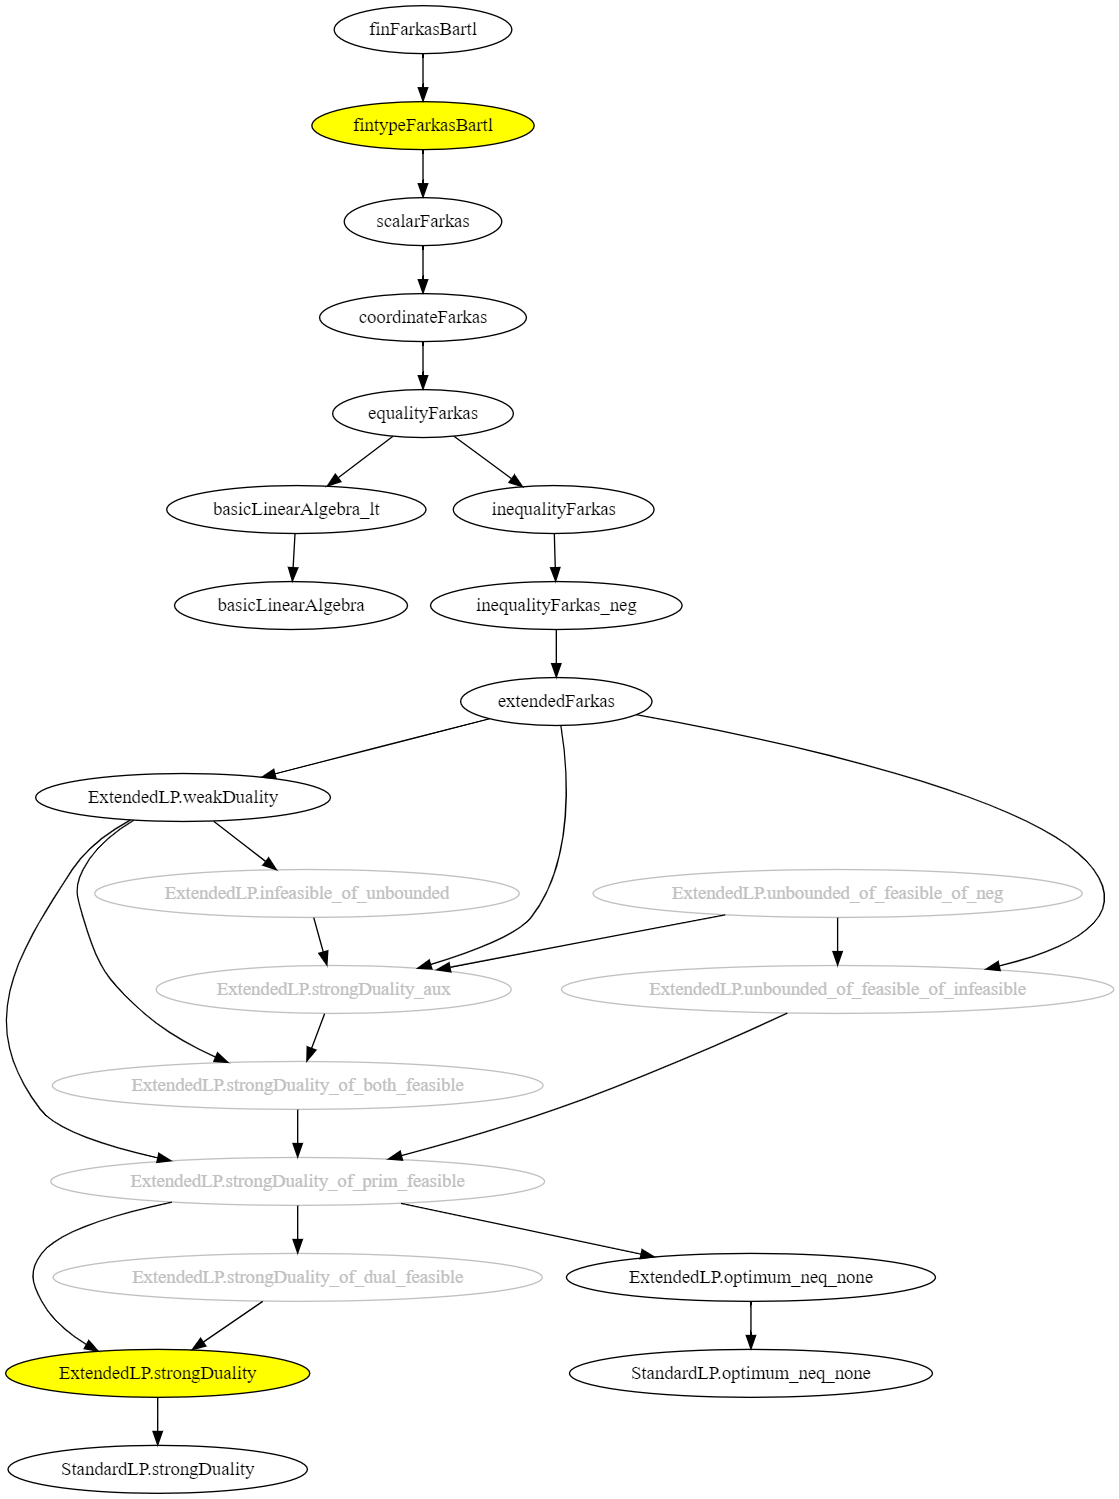
\includegraphics[width=0.9\textwidth]{theorems.png}


\end{document}
